\documentclass[12pt,twoside]{article}
\usepackage{hyperref} 
\usepackage{fixltx2e}
\usepackage{minted}
\usepackage{verbatim}
\usepackage{graphicx}

\newcommand{\doctitle}{%
Universal Cycles}

\pagestyle{myheadings}
\markboth{\hfill\doctitle}{\doctitle\hfill}

\bibliographystyle{siam}

\addtolength{\textwidth}{1.00in}
\addtolength{\textheight}{1.00in}
\addtolength{\evensidemargin}{-1.00in}
\addtolength{\oddsidemargin}{-0.00in}
\addtolength{\topmargin}{-.50in}

\hyphenation{in-de-pen-dent}

\title{\textbf{\doctitle}\\
CS7083 Final Project Report}

\author{Jayanth Dungavath}

\begin{document}
\maketitle
\pagebreak



\hfill \break
\hfill \break
\hfill \break
\hfill \break
\hfill \break
\hfill \break
\hfill \break
\hfill \break
\hfill \break
\hfill \break
\hfill \break
\hfill \break
\hfill \break
\hfill \break
\hfill \break
\hfill \break
\hfill \break
\hfill \break
\hfill \break
\hfill \break
\hfill \break
\hfill \break
\hfill \break
\hfill \break
\hfill \break
\hfill \break
\pagebreak

\tableofcontents
%\thispagestyle{empty}


\hfill \break
\hfill \break
\hfill \break
\hfill \break
\hfill \break
\hfill \break
\hfill \break
\hfill \break
\hfill \break
\hfill \break
\hfill \break
\hfill \break
\hfill \break
\hfill \break
\hfill \break
\hfill \break
\hfill \break
\hfill \break
\hfill \break
\hfill \break
\hfill \break
\hfill \break
\hfill \break
\hfill \break

%\section{Environment}
%\begin{itemize}
%    \item \textbf{OS}: Elementary OS Luna
%    \item \textbf{Languages}: Python 3.0, C
%    \item \textbf{Processor}: Intel Core 2 Duo, 2.2 GHz
%    \item \textbf{Memory}: 4GB 800 MHz DDR2 SDRAM
%    \item \textbf{Editor}: Emacs
%    \item \textbf{Documentation}: TeXShop (Mac OS X)
%\end{itemize}


\graphicspath{ {/Users/jayanthdeejay/Documents/Edu/UC/Classes/Combinatorics/project/} }

\section{Abstract}
The aim of this project is to implement and better understand the construction of de Bruijn Sequences and Universal Cycles using various algorithms like FKM algorithm by Fredricksen, Kessler and Maiorana (FKM) proposed in Fredricksen and Kessler \cite{FK} and in Fredricksen and Maiorana \cite{FM} and J. P. Duval  \cite{Duval} proposed an algorithm to produce Lyndon words and subsequently producing Universal Cycles. The study of these cycles has arisen in a variety of contexts like digital fault testing, pseudo-random number generations etc., there by triggering interest among researchers producing extensive results in these fields.


\section{Introduction}
\subsection{de Bruijn Sequence}
Let \textbf{T}(\emph{n, k}) be the set of \emph{k}-ary strings of length \emph{n}. A de Bruijn sequence for \textbf{T}(\emph{n, k}) is a sequence of length $k^n$ that contains each string in \textbf{T}(\emph{n, k}) exactly once as a substring when the sequence is viewed circularly \cite{Sawada}. For Example, \[\textbf{T}(2, 3) = \{11, 12, 13, 21, 22, 23, 31, 32, 33\}\]
M. H. Martin's greedy algorithm \cite{Martin} can construct a de Bruijn sequence for \textbf{T}(\emph{n, k}) by starting a sequence with $k^{n-1}$ (exponent denotes repetition of $k$ by $n-1$ times) and repeatedly applying the following rule:
\begin{center} \emph{Append the smallest symbol in} \{1,2,...,k\} \emph{so that substrings of length n in the resulting linear sequence are distinct.} \end{center}
When $\emph{n}=2$ and $\emph{k}=3$, the algorithm generates 3112132233 and a de Bruijn sequence is obtained by removing the initial $k^{n-1}$ prefix. So, 112132233 is a de Bruijn Sequence for \emph{T}(2, 3). Though Martin's algorithm is easy to implement, it is a space complex algorithm taking $\Omega(k^n)$ space. An alternative, FKM algorithm is both space and time efficient algorithm and is discussed in a separate section. 

\subsection{Universal Cycles}
Chung, Diaconis, and Graham in 1992 \cite{Chung} have introduced the natural generalization of de Bruijn sequences for \textbf{T}(\emph{n, k}) to subsets of \textbf{T}(\emph{n, k}). Given a set of strings \textbf{S} $\subseteq$ \textbf{T}(\emph{n, k}), a universal cycle for \textbf{S} is a sequence of length $\mid$\textbf{S}$\mid$ that contains each string in \textbf{S} exactly once as a substring when the sequence is viewed circularly. For example, the subset \textbf{S\textsubscript{1}}  $\subseteq$  \textbf{T}(4, 3) of strings that have sum at least 10 is \begin{center} \textbf{S\textsubscript{1}} = \{1333,2233,2323,2332,2333,3133,3223,3232,3233,3313,3322,3323,3331,3332,3333\} \end{center}

The universal cycle for \textbf{S\textsubscript{1}} is \begin{center} 133322332323333 \end{center}

\section{FKM Algorithm}
FKM algorithm can be summarized as follows: \begin{center} \emph{Concatenate the aperiodic prefixes of the necklaces in} \textbf{T}(\emph{n, k}) \emph{in lexicographic order}\end{center}
For example, \\ \\\textbf{T}(4,2) = \{0000, 0001, 0010, 0011, 0100, 0101, 0110, 0111, 1000, 1001, 1010, 1011, 1100, 1101, 1110, 1111\}

As the strings are already in lexicographic order, we need to find the aperiodic prefixes of the necklaces in \textbf{T}(\emph{n, k}). A necklace or a Lyndon word can be defined as the lexicographically smallest string in an equivalence class strings under rotation. And, its aperiodic prefix is the shortest prefix that can be repeated to create the string itself. Following are the necklaces and their aperiodic prefixes of \textbf{T}(\emph{n, k}):
\begin{center}
\begin{tabular}{ c c }
 \textbf{Necklace} & \textbf{Aperiodic Prefix} \\ 
 0000 & 0 \\  
 0001 & 0001 \\
 0011 & 0011 \\
 0101 & 01 \\
 0111 & 0111\\
 1111 & 1\\    
\end{tabular}
\end{center}
Concatenation of these aperiodic prefixes gives \begin{center}$0\cdot0001\cdot0011\cdot01\cdot0111\cdot1$\end{center}
Universal cycle 0000100110101111 contains each strings in \textbf{T}(4, 2) exactly once as a substring when it is viewed circularly. FKM algorithm always generates the same sequence for the given \emph{n, k}.

\section{J. P. Duval Algorithm}
Duval in 1988 has given an algorithm that produces Lyndon words of length less than or equal to an integer n \cite{Duval}. By concatenating the generated Lyndon words, we can get a Universal Cycle. Though the actual paper is not in English, I found the pseudo code of the algorithm \cite{Chemillier} and implemented the same. 
\hfill \break
\hfill \break
\hfill \break
\hfill \break
\hfill \break
\hfill \break

\textbf{Algorithm is as follows:} \\

\noindent\rule{16.5cm}{1.0pt}
1: w[1] $\leftarrow$ a\\
2: i $\leftarrow$ 1\\
3: \textbf{repeat}\\
4: \hspace{0.5cm} \textbf{for} $j = 1$ to $n - i$\\
5: \hspace{1.0cm} \textbf{do} $w[i+j] \leftarrow w[j]$\\
6: \hspace{0.5cm} $i \leftarrow n$\\
7: \hspace{0.5cm} \textbf{while} $i > 0$ \textbf{and} $w[i] = M$\\
8: \hspace{1.0cm} \textbf{do} $i \leftarrow (i - 1)$\\
9: \hspace{0.5cm} \textbf{if} $i > 0$ \\
10: \hspace{1.0cm} \textbf{then} $w[i] \leftarrow s(w[i])$\\
11: \textbf{until} $i = 0$\\
\noindent\rule{16.5cm}{1.0pt}
Letters a and M are respectively the first and last letters of the alphabet, and for every letter x excepted M, s(x) is the letter that follows x in the alphabet. We denote by w[1...n] an array of letters of dimension n. \\
\section{Implementation}
After completing the research and review of necessary material required for this project, I started implemeting these algorithms in Python. One entire module had been dedicated to implement FKM and another one to implement Duval's algorithm. Code samples are documented in the following section.


\subsection{FKM algorithm implementation:}
Implemented this algorithm based on the algorithm's description provided in \cite{Sawada}. Initially, all the words of length n are generated from the set of symbols s. Then necklaces are identified to later produce aperiodic prefixes which are then joined to produce a universal cycle. \\ 
\hfill \break
\hfill \break
\hfill \break
\hfill \break
\hfill \break
\hfill \break
\hfill \break
\hfill \break
\hfill \break
Following universal cycle has been generated for $s$ = \{1, 2, 3\} and $n = 4$ with strings that have sum at least 10.\\
\noindent\rule{16.5cm}{1.0pt}
-bash-4.1\$ python FKM.py\\
String: 123\\
Length: 4\\
1. De Bruijn Sequence\\
2. Universal Cycle\\
1/2? 2\\
Enter val such that each string has sum at least val: 10\\
\textbf{Universal cycle: 133322332323333}\\
-bash-4.1\$ \\
\noindent\rule{16.5cm}{1.0pt} \\ \\

\textbf{Code:}
\begin{minted}[linenos=true]{python}
def toString(List):
    return ''.join(List)

strings = []
def stringPermutations (strng, dat, lst, idx):
    length = len(strng)
    for i in range(length):
        dat[idx] = string[i]
        if idx==lst:
            strings.append(toString(dat))
        else:
            stringPermutations (strng, dat, lst, idx+1)

def generateStrings (strng, length):
    global strings
    strings = []
    dat = [""] * (length+1)
    strng = sorted(strng)
    stringPermutations (strng, dat, length-1, 0)

def necklaces(p):
    for i in p:
        for j in range(1,len(i)):
            if (not(i[1:]+i[:1]==i)):
                x = i[j:]+i[:j]
                if x in p:
                    if (not(i==x)):
                        p.remove(x)
    return p

def atleast(x,val):
    p = []
    for i in x:
        sum = 0
        for j in i:
            sum += int(j)
        if (sum >= val):
            p.append(i)
    return p

def aperiodic(p):
    prefix = []
    for i in p:
        if(len(i)%2 == 0):
            if(i[1:]+i[:1]==i):
                prefix.append(i[:1])
            elif(i[:2]*(len(i)/2)==i):
                prefix.append(i[:2])
            elif(i[:len(i)/2]*2==i):
                prefix.append(i[:len(i)/2])
            else:
                prefix.append(i)
        elif(len(i)==9):
            if(i[1:]+i[:1]==i):
                prefix.append(i[:1])
            elif(i[:3]*3==i):
                prefix.append(i[:3])
            else:
                prefix.append(i)
        else:
            if(i[1:]+i[:1]==i):
                prefix.append(i[:1])
            else:
                prefix.append(i)
    return prefix
    
strng = raw_input("String: ")
length = input("Length: ")
generateStrings(strng, length)
strings = necklaces(strings)
strings = aperiodic(strings)
strings = "".join(strings)
print strings

\end{minted}




\subsection{Duval algorithm implementation:}
Implemented two variations of this algorithm. One version, given $s = 3$ and $n = 2$ produces the following universal cycle.
\begin{equation} \label{eq:1}
[1, 1, 2, 1, 3, 2, 2, 3, 3]
\end{equation}
And the other implementation produces following universal cycle.
\begin{equation} \label{eq:2}
[0, 0, 1, 0, 2, 1, 1, 2, 2]
\end{equation} 
Notice the change in the range of symbols. Former implementation considers s = \{1, 2, 3\} and latter implementation considers s = \{0, 1, 2\}. \\ \\
\textbf{Code}
\begin{minted}[linenos=true]{python}
def lyndonWords(s,n):
    strings = [0] #strings = [-1]
    while strings:
        strings[-1] += 1
        yield strings
        los = len(strings)
        while len(strings) < n:
            strings.append(strings[-los])
        while strings and strings[-1] == s: 
        #while strings and strings[-1] == s - 1: 
            strings.pop()

def uCycle(s,n):
    cycle = []
    for c in lyndonWords(s,n):
        if n % len(c) == 0:
            cycle += c
    return cycle

\end{minted}
Universal cycle in list \ref{eq:1} is generated using this particular implementation. Replacing the commented code with the respective lines produces the universal cycle list \ref{eq:2}.

\hfill \break
\hfill \break
\hfill \break
\section{Results}
The implemented code works and they do generate the universal cycles as intended with drawbacks in each algorithm. Duval's algorithm is supposed to yield an overall running time of $\mathcal{O}(nN(n))$ \cite{Berstel}, where N(n) stands for the number of necklaces over n. Time complexity of my implementation seems to complement the theory but the space complexity is really high. \\

To generate a universal cycle for given $s = 9, n = 9$, the program used a total of 6.382 GB space. But, it only took \url{~}46 seconds. On the other hand, FKM algorithm consumes negligible space when it is compared to the Duval algorithm, but the algorithm is extremely slow. Given $s = 7, n = 7$, it took my FKM program over 6922 secs and Duval only 0.138 secs. After doing further research, I came to conclude that my FKM implementation isn't efficient. I found pseudo code of FKM algorithm \cite{Savage} which when implemented might be even more efficient. Based on my sample runs on OSC Supercomputing Oakley Cluster, I generated graphs in figure \ref{fig:exectimes}, \ref{fig:duval} and \ref{fig:fkm}.

\begin{figure}
  \centering
    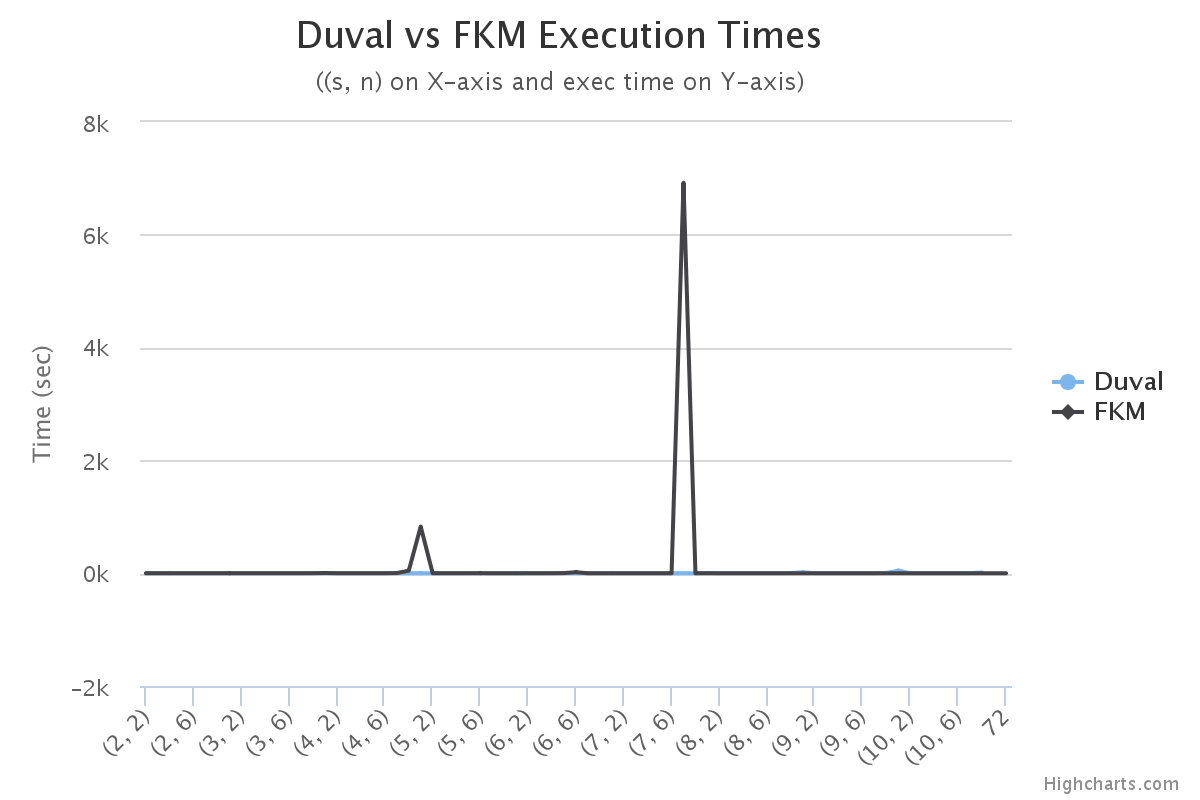
\includegraphics[width=6in]{exectimes.png}
  \caption{Duval vs FKM}
  \label{fig:exectimes}
\end{figure}
\\
\textbf{Interactive graphs of figure \ref{fig:exectimes}, \ref{fig:duval} and \ref{fig:fkm} can be viewed by clicking \href{http://homepages.uc.edu/~dungavjk/webres/work/exectimes.html}{here}}. \\

\begin{figure}
  \centering
    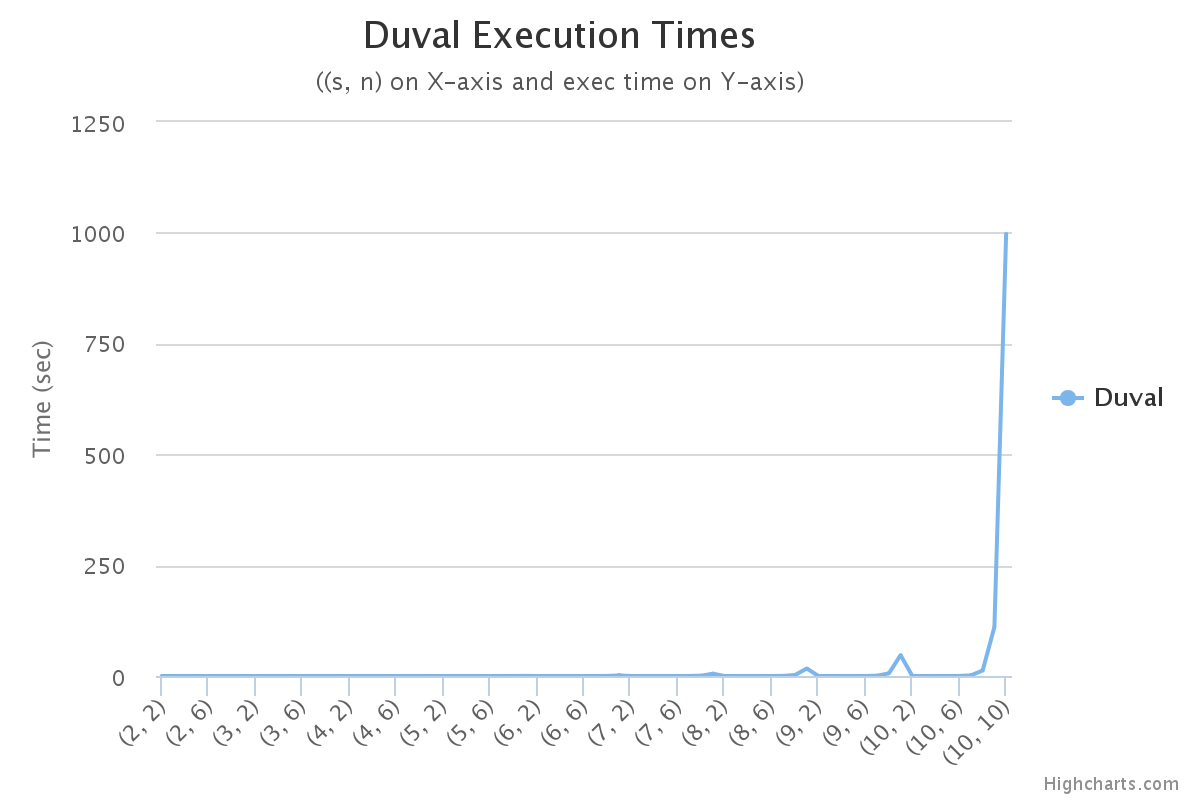
\includegraphics[width=6in]{duval.png}
  \caption{Duval Algorithm}
  \label{fig:duval}
\end{figure}


\begin{figure}
  \centering
    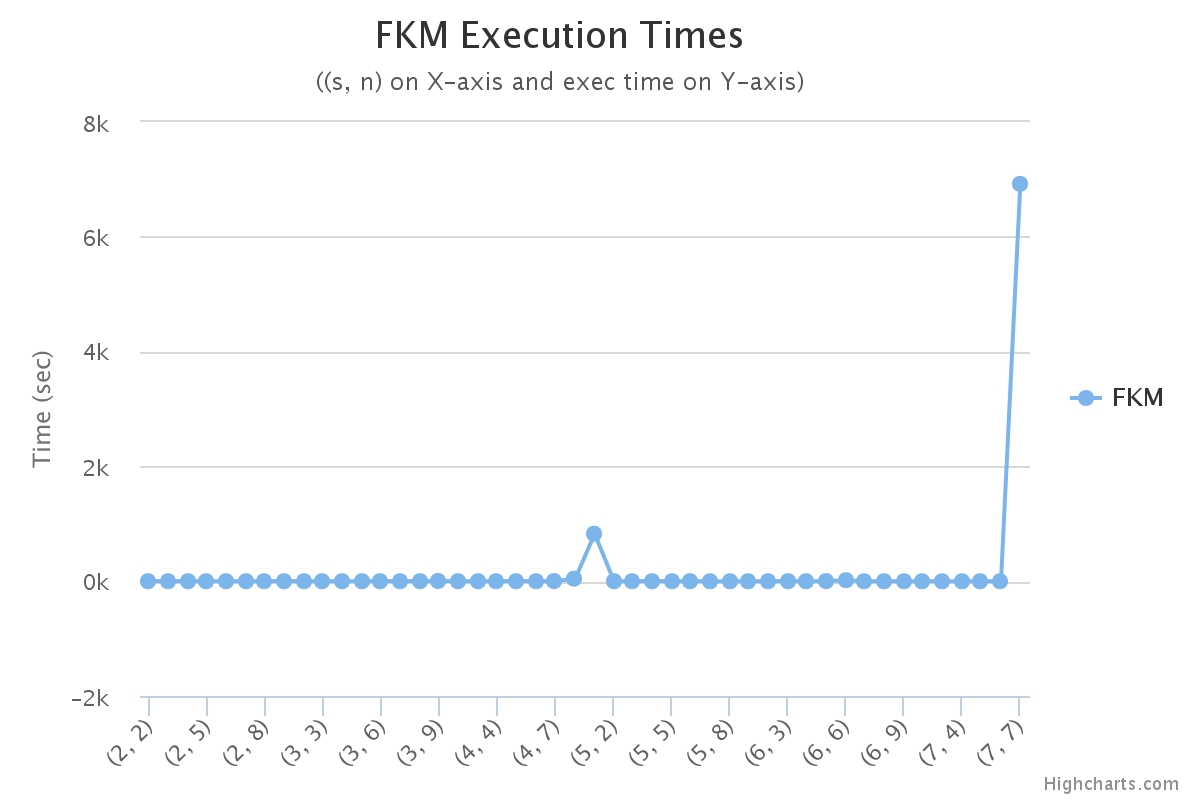
\includegraphics[width=6in]{fkm.png}
  \caption{FKM Algorithm}
  \label{fig:fkm}
\end{figure}
\hfill \break

\section{Conclusion and Future work}
Working on this project has helped in broadening my horizon and also gave me a research direction for my thesis work. Looking forward to further modify the implementations such that they are both time and space efficient. Also came across some interesting papers. Dong and Pei \cite{Dong} have presented an algorithm for constructing de Bruijn sequences with large orders (such as $n = 128$). Also, there is another interesting paper by Diaconis and Graham \cite{Graham} where in they show how to construct a \textbf{product cycle} of two universal cycles.

\begin{thebibliography}{9}
\bibitem{FK} 
H. Fredricksen and I. J. Kessler,
\textit{An algorithm for generating necklaces of beads in two colors},
Discrete Mathematics 61 (1986), 181-188.

\bibitem{FM} 
H. Fredricksen and J. Maiorana,
\textit{Necklaces of beads in k colors and k-ary de Bruijn sequences},
Discrete Mathematics 23 (1978), 207-210.

\bibitem{Duval} 
J. P. Duval,
\textit{Generation d'une section des classes de conjugaison et arbre des mots de Lyndon de longueur bornee},
Theoretical Computer Science archive, Volume 60 Issue 3, September 1988 Pages 255 - 283.

\bibitem{Sawada} 
Joe Sawada, Aaron Williams and Dennis Wong,
\textit{Generalizing the Classic Greedy and Necklace Constructions of de Bruijn Sequences and Universal Cycles},
The Electronic Journal of Combinatorics 23(1) (2016), \#P1.24.


\bibitem{Martin} 
M. H. Martin,
\textit{A problem in arrangements},
Bulletin of the American Mathematical Society, 40:859?864, 1934.


\bibitem{Chung} 
Chung, F., P. Diaconis and R. Graham,
\textit{Universal cycles for combinatorial structures},
Discrete Mathematics 110 (1992) 43-59.


\bibitem{Chemillier} 
Marc Chemillier,
\textit{Periodic musical sequences and Lyndon words},
Soft Computing, 8:611?616, 2004.


\bibitem{Berstel} 
Berstel, J. and M. Pocchiola,
\textit{Average cost of Duval?s algorithm for generating Lyndon words},
Theoretical Computer Science 132 (1994) 415-425. 


\bibitem{Savage} 
F. Ruskey, C. D. Savage, and T. Wang,
\textit{Generating necklaces},
J. Algorithms, 13 (1992), pp. 414?430


\bibitem{Dong} 
J. Dong and D. Pei,
\textit{Construction for de Bruijn sequences with large orders},
Cryptology ePrint Archive: Report 2015/1091.


\bibitem{Graham} 
P. Diaconis and R. L. Graham,
\textit{Products of universal cycles},
A Lifetime of Puzzles, E. Demaine, M. Demaine and Tom Rodgers, eds., A K Peters, 2008, Boston, MA pp. 35?55.


\end{thebibliography}















\end{document}